\documentclass[final]{beamer}
\usepackage{color}
\usetheme{RJH}
\usepackage[orientation=portrait,size=a1,scale= 1.8,debug]{beamerposter}
\usepackage[absolute,overlay]{textpos}
\usepackage{animate}

\usepackage{fancyhdr}
\usepackage{apacite}


%\usepackage[usenames,dvipsnames]{xcolor}
\setlength{\TPHorizModule}{1cm}
\setlength{\TPVertModule}{1cm}

\title{{\LARGE Extending Bayesian analysis of circular data \\ to comparison of multiple groups}}
\author{{\large Kees Mulder} \\ {  \normalsize  Utrecht University }}
\footer{}

\definecolor{keesred}{RGB}{222,45,38}

\begin{document}
\begin{frame} 

%%%%%%%%%%%%%%%%%%%%%%%%%%%%%%%%%%%%%%%%%%%%%%%%%%%%%%%%%%%
%
\begin{textblock}{55}(2,8)


\begin{block}{\centering What is circular data?}
\textbf{Circular} data have a \textbf{periodical} sample space.

They may be \textbf{angles}, \textbf{directions} or \textbf{orientations}, measured in \textbf{radians}, \textbf{degrees}, or  \textbf{unit vectors}. 

%Denote a datum by $\theta$, and the sample space by $\mathbb{S}^1$.

\vspace{1cm}

\begin{minipage}{0.55\textwidth}

Examples are found in a large variety of disciplines:

\begin{itemize}
\item The direction of animal movement. 
\item The orientation of fractures in rocks.
\item The time of day, or day of the year.
\item Measurements on a circumplex model, such as Leary's rose for interpersonal behaviour. 
\item Parts of the structure of proteins and DNA.
\end{itemize}
\end{minipage}
\begin{minipage}{0.20\textwidth}
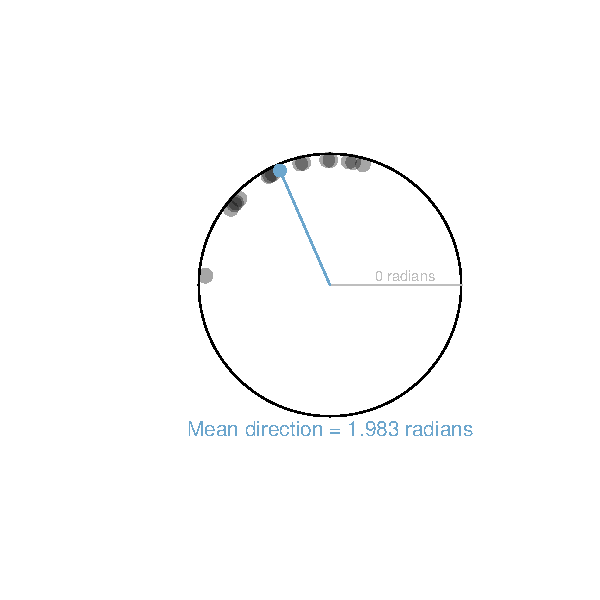
\includegraphics[width=\textwidth, trim = 2.8cm 2.5cm 2.1cm 2.6cm, clip]{Exampledataset1.pdf}
\end{minipage}
\begin{minipage}{0.20\textwidth}
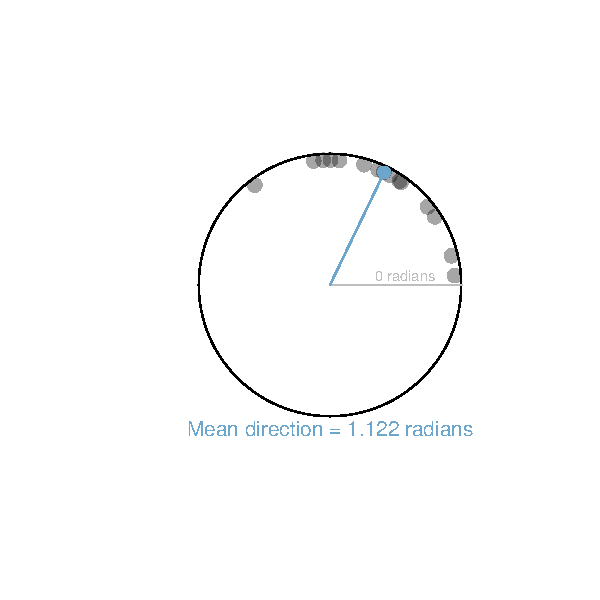
\includegraphics[width=\textwidth, trim = 2.8cm 2.5cm 2.1cm 2.6cm, clip]{Exampledataset2.pdf}
\end{minipage}
\vspace{1cm}

Specialized methods for circular data are necessary. Here, we focus on models with a \textbf{circular outcome}.

\end{block}
%
\end{textblock}
\begin{textblock}{26.5}(2,27)
%
\vspace{\TPHorizModule}

\begin{block}{The problem}

\begin{itemize}
\item Circular data are \textbf{inherently difficult to analyze}, due to the circular sample space.
\item \textbf{Few methods} have been developed for circular outcomes.
\item Bayesian methods, especially MCMC, offer a promising new route for circular data models. 
%\item Current theoretical work lacks applied solutions. 
\item Focusing on the \textbf{circular ANOVA} context: \textcolor{keesred}{There is currently no Bayesian model for testing \textbf{group mean differences}, assuming \textbf{equal variance}.}
\item Equal variance here means that the \textbf{concentration parameter $\kappa$} should be \textbf{equal across groups}.
\end{itemize}
\end{block}

\vspace{\TPHorizModule}

\begin{block}{Circular data approaches}
\begin{itemize}
\item The \textbf{intrinsic} approach, directly defined on the circle, for example using the von Mises distribution
$$ \mathcal{VM}(\theta \vert \mu, \kappa) \propto \exp\left[ \kappa \cos (\theta - \mu) \right].$$
\item The \textbf{wrapping} approach, where distributions in $\mathbb{R}^1$ are wrapped around the circle. 
\item The \textbf{embedding} approach, embedding points in $\mathbb{R}^2$ to the circle.
\end{itemize}

Here, we employ the \textbf{intrinsic approach}.

\end{block}



\vspace{\TPHorizModule}
\begin{block}{Conditionals}
\begin{small}
A conjugate prior for von Mises is available, which uses $\boldsymbol{\mu_{0}}, R_0, c$. For an uninformative prior, we set $R_0 = 0, c = 0$. Then, given data $\boldsymbol{\theta}$:
$$ C_n = R_0 \cos \mu_0 + \sum_{i=1}^n \cos \theta_i, ~~~~ S_n = R_0 \sin \mu_0 + \sum_{i=1}^n \sin \theta_i,$$
$$  \mu_n = \text{atan2}(S_n/C_n,) $$
$$ R_n = \sqrt{C_n^2 + S_n^2}.$$
The conditionals are then:
\begin{align*}
f(\mu_j \vert \kappa, \boldsymbol\theta) & = \mathcal{VM}(\mu_{nj}, R_{nj} \kappa) \propto \exp\{R_{nj} \kappa \cos(\mu - \mu_{nj})\},\\
f(\kappa \vert \mu, \boldsymbol\theta) &\propto \{ I_0(\kappa) \} ^{-(n+c)} \exp\left[  R_n \kappa \sum_{j=1}^{J}\cos(\mu - \mu_{nj}) \right]. 
\end{align*}
\end{small}
\end{block}


\end{textblock}
%
%%%%%%%%%%%%%%%%%%%%%%%%%%%%%%%%%%%%%%%%%%%%%%%%%%%%%%%%%%%%
%
\begin{textblock}{26.5}(30.5,27)
\vspace{\TPHorizModule}
%\begin{block}{Between-subjects analysis}
%\begin{itemize}
%\item We usually \textbf{assume homogeneity of variance.}
%\item In our approach, we use a concentration parameter $\kappa$ as a measure of spread.
%\item Under the current methods, it is \textbf{not possible to sample from the posterior with multiple groups} with common concentration parameter.
%\end{itemize}
%Thus, the \textbf{existing methods were extended.}
%\end{block}

%\vspace{\TPHorizModule}
\begin{block}{Intrinsic methods}
Three solutions were developed:
\begin{itemize}
\item A \textbf{Gibbs sampler} using auxiliary variables, extending Damien \& Walker (1999).
\item A \textbf{Metropolis-Hastings} method.
\item A recent \textbf{rejection sampling} method, extending Forbes \& Mardia (2014).
\end{itemize}
\end{block}

\vspace{\TPHorizModule}

\begin{block}{Comparison of the three methods}
%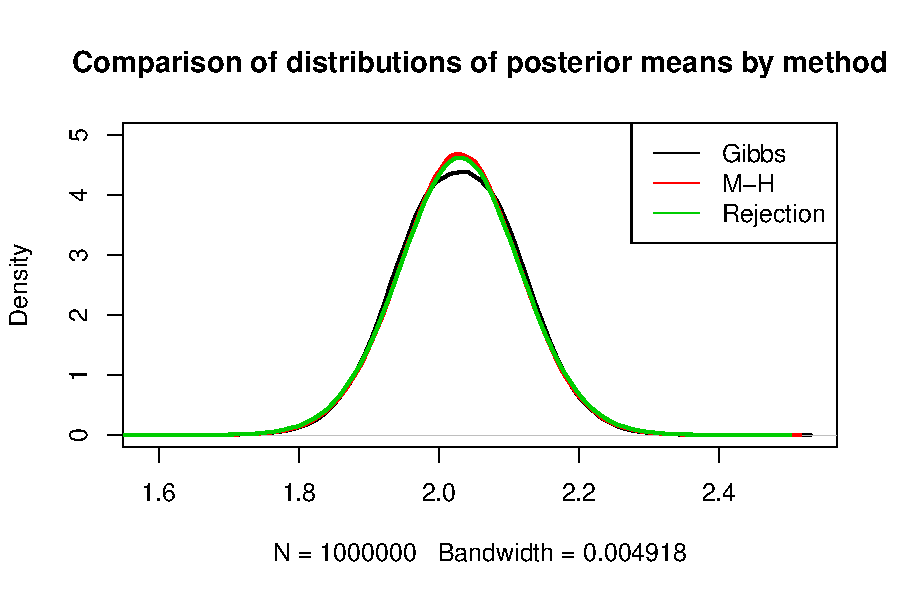
\includegraphics[width=0.49\textwidth, trim = 0cm 1.5cm 0cm 0cm, clip]{MeanComparison.pdf}
%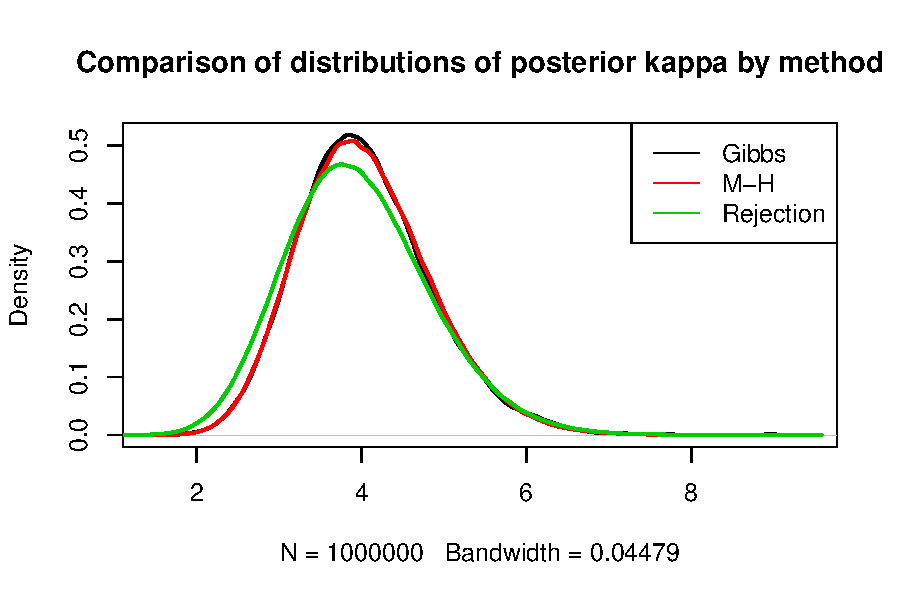
\includegraphics[width=0.49\textwidth, trim = 0cm 1.5cm 0cm 0cm, clip]{KapComparison.pdf}
\begin{center}
\includegraphics[width=0.8\textwidth, trim = 1.3cm 1.5cm 0cm 0.5cm, clip]{ExampleRun.pdf}
\end{center}

The Gibbs sampler encounters strong autocorrelation when roughly $\kappa > 7.$ 

Coverage for $\kappa:$
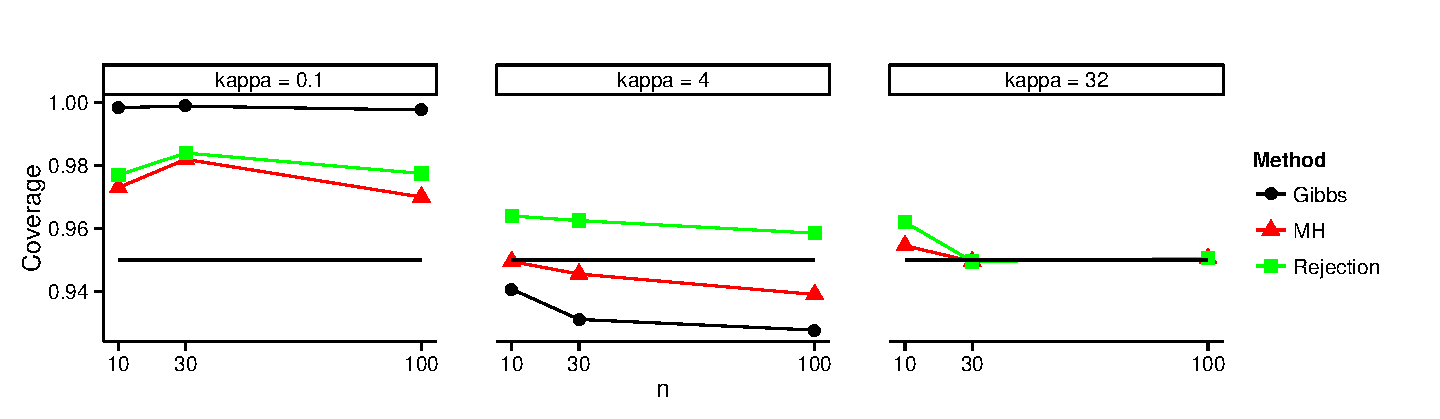
\includegraphics[width=\textwidth]{CoveragesWide.pdf}

The MH and rejection samplers performed well, with the rejection sampler being slightly more efficient.  

\end{block}


\vspace{\TPHorizModule}

\begin{block}{Contact}
\begin{small}
This poster was supported by an ISBA travel grant.

Kees Mulder \& I. Klugkist\\
Utrecht University \\
\url{k.t.mulder@uu.nl}\\
\url{i.klugkist@uu.nl}
\end{small}
\vspace{-0.5cm}
\end{block}
%\begin{block}{References}
%\begin{footnotesize}
%
%\bibliographystyle{apacite}
%\bibliography{C:/Dropbox/Masterthesis/Writing/CircularData}
%\end{footnotesize}
%
%\end{block}
%
\end{textblock}
\end{frame}

\end{document}
